% $Header: /Users/joseph/Documents/LaTeX/beamer/solutions/conference-talks/conference-ornate-20min.en.tex,v 90e850259b8b 2007/01/28 20:48:30 tantau $

\documentclass{beamer}
\usepackage{graphicx}
% This file is a solution template for:

% - Talk at a conference/colloquium.
% - Talk length is about 20min.
% - Style is ornate.



% Copyright 2004 by Till Tantau <tantau@users.sourceforge.net>.
%
% In principle, this file can be redistributed and/or modified under
% the terms of the GNU Public License, version 2.
%
% However, this file is supposed to be a template to be modified
% for your own needs. For this reason, if you use this file as a
% template and not specifically distribute it as part of a another
% package/program, I grant the extra permission to freely copy and
% modify this file as you see fit and even to delete this copyright
% notice. 


\mode<presentation>
{
  \usetheme{Madrid}
  % or ...
\usecolortheme{beaver}
  \setbeamercovered{transparent}
  \setbeamerfont{section number projected}{%
  family=\rmfamily,series=\bfseries,size=\normalsize}
  \setbeamercolor{section number projected}{bg=gray,fg=white}
    \usefonttheme{professionalfonts} 
    \setbeamertemplate{itemize item}{\color{gray}$\bullet$}
     \setbeamertemplate{enumerate items}[default]
    \setbeamercolor*{enumerate subitem}{fg=black}
   \setbeamercolor{caption name}{fg=structure!10!black}
   \setbeamercolor{bibliography entry author}{fg=red}
   \setbeamercolor{bibliography entry location}{fg=gray}
}

\usepackage{verbatim}
\usepackage[english]{babel}
% or whatever

\usepackage[latin1]{inputenc}
% or whatever

\usepackage{times}
\usepackage[T1]{fontenc}
% Or whatever. Note that the encoding and the font should match. If T1
% does not look nice, try deleting the line with the fontenc.


\title[Manifold Mapping] % (optional, use only with long paper titles)
{Numerically Solving PDEs \\While Mapping Between Manifolds}


\author[King] % (optional, use only with lots of authors)
{\vspace{1cm}\\
Nathan King}
% - Give the names in the same order as the appear in the paper.
% - Use the \inst{?} command only if the authors have different
%   affiliation.

\institute[SFU] % (optional, but mostly needed)
{
  Department of Mathematics\\
Simon Fraser University\\
 }
% - Use the \inst command only if there are several affiliations.
% - Keep it simple, no one is interested in your street address.

\date[June 23, 2014] % (optional, should be abbreviation of conference name)
{June 23, 2014}
% - Either use conference name or its abbreviation.
% - Not really informative to the audience, more for people (including
%   yourself) who are reading the slides online

\subject{Numerical Analysis}
% This is only inserted into the PDF information catalog. Can be left
% out. 



% If you have a file called "university-logo-filename.xxx", where xxx
% is a graphic format that can be processed by latex or pdflatex,
% resp., then you can add a logo as follows:

% \pgfdeclareimage[height=0.5cm]{university-logo}{university-logo-filename}
% \logo{\pgfuseimage{university-logo}}




\usepackage{amsmath}
\usepackage{tikz}
\newcommand\diag[4]{%
  \multicolumn{1}{p{#2}|}{\hskip-\tabcolsep
  $\vcenter{\begin{tikzpicture}[baseline=0,anchor=south west,inner sep=#1]
  \path[use as bounding box] (0,0) rectangle (#2+2\tabcolsep,\baselineskip);
  \node[minimum width={#2+2\tabcolsep},minimum height=\baselineskip+\extrarowheight] (box) {};
  \draw (box.north west) -- (box.south east);
  \node[anchor=south west] at (box.south west) {#3};
  \node[anchor=north east] at (box.north east) {#4};
 \end{tikzpicture}}$\hskip-\tabcolsep}}




% If you wish to uncover everything in a step-wise fashion, uncomment
% the following command: 

%\beamerdefaultoverlayspecification{<+->}

\DeclareMathOperator*{\argmin}{arg\,min}
\begin{document}
  
  
  
\begin{frame}
  \titlepage
\end{frame}


% Structuring a talk is a difficult task and the following structure
% may not be suitable. Here are some rules that apply for this
% solution: 

% - Exactly two or three sections (other than the summary).
% - At *most* three subsections per section.
% - Talk about 30s to 2min per frame. So there should be between about
%   15 and 30 frames, all told.

% - A conference audience is likely to know very little of what you
%   are going to talk about. So *simplify*!
% - In a 20min talk, getting the main ideas across is hard
%   enough. Leave out details, even if it means being less precise than
%   you think necessary.
% - If you omit details that are vital to the proof/implementation,
%   just say so once. Everybody will be happy with that.

\begin{frame}{Overview of Research}
\begin{itemize}
\item Research involves numerical methods for solving PDEs (and variational problems) defined on surfaces.
\item Work with are embedding methods, which embed the surface PDE in a higher dimensional space.
\item For example, a PDE defined on a sphere is embedded in $\mathbb{R}^3.$
\item Embedding methods allow for standard, well studied numerical methods on cartesian grids to be used.
%\item Other approaches are: 1) parametrize (impose a smooth coordinate system) the surface and express differential operators in this parametrization. 2) solve the PDE directly on a triangulation of the surface. %(know problems with these if asked!)
\end{itemize}
\end{frame}

\begin{frame}{Outline}
     \tableofcontents
\end{frame}

\section{Level Set Method}
\begin{frame}{Level Set Method}
\begin{itemize}
\item Level Set method illustrated with heat equation on a surface $\mathcal{S}.$
\item Heat equation defined on $\mathcal{S}$ is $$\frac{\partial u}{\partial t} =\Delta_{\mathcal{S}} u.$$
\item Embed $\mathcal{S}$ using a level set function $\phi : \mathbb{R}^3 \rightarrow \mathbb{R}.$ 
\item Zero level set represents $\mathcal{S},$ that is $\mathcal{S} = \{\phi = 0\}.$
\item Take $\phi$ to be the signed distance function of $\mathcal{S}.$ 
\item Signed distance function has property that $\|\nabla \phi\| = 1.$
\end{itemize}
\end{frame}


\begin{frame}{Level Set Method}
\begin{itemize}
\item  Intrinsic gradient of $u$ on $\mathcal{S}$ can be written in terms of gradients in $\mathbb{R}^3,$  $$\nabla_{\mathcal{S}} u = \mathcal{P}_{\nabla \phi} \nabla u.$$

\item Operator $$\mathcal{P}_v=I-\frac{v \hspace{0.1cm} v^T}{\| v \|^2}$$ projects any given vector into a plane orthogonal to $v.$

\item Heat equation on $\mathcal{S}$ becomes $$\frac{\partial u}{\partial t} =\nabla \cdot(\mathcal{P}_{\nabla \phi} \nabla u),$$ which is now defined in $\mathbb{R}^3.$

\end{itemize}
\end{frame}


\section{Closest Point Method}
\begin{frame}{Closest Point Method}
\begin{itemize}
\item Want to create embedding PDE which replaces intrinsic surface gradients with standard gradients.
\item Obviously the embedding PDE and surface PDE will not agree for long times, however this is accurate initially and is sufficient to update the solution in time.
\item A closest point representation of the surface is used.
\item For any point ${\bf x}\in \mathbb{R}^3,$ let $CP({\bf x}$) denote the closest point to ${\bf x}$ in $\mathcal{S}.$ 
\item $CP$ is a function from $\mathbb{R}^3$ to $\mathbb{R}^3$ that returns values lying in $\mathcal{S}.$ 
%
%\item Extension operator extends functions defined on the surface constant normal to the surface.
%\item A simple, accurate and efficient method for a constant normal extension makes use of the closest point representation of the surface.
\end{itemize}
\end{frame}

\begin{frame}{Closest Point Method}
\begin{itemize}
\item Embed the surface PDE by replacing surface gradients, $\nabla_{\mathcal{S}},$ with standard gradients, $\nabla,$ in $\mathbb{R}^3.$
\item Alternate between two steps:
\begin{enumerate}
\item Extend surface data into $\mathbb{R}^3$ using the closest point function, i.e. replace $u({\bf x})$ with $u(CP({\bf x})).$
\item Compute solution to embedding PDE using standard finite differences on Cartesian grid for one time step.
\end{enumerate}
\end{itemize}
\end{frame}

\section{Extension of Level Set Method with Manifold Mapping}
\begin{frame}{Mapping Between Manifolds}
\begin{itemize}
\item Let $\mathcal{M}$ denote the source manifold and $\mathcal{N}$ the target manifold.
\item Signed distance functions of $\mathcal{M}$ and $\mathcal{N}$ are $\phi$ and $\psi,$ respectively.
\item Goal is to compute a vector function $u : \mathcal{M} \rightarrow \mathcal{N}$ that minimizes $$E=\frac{1}{2} \int \|\mathcal{P}_{\nabla \phi} \nabla u \|^2 \; \delta (\phi) d\mathcal{M}. $$ 
\item Gradient descent flow is $$\frac{\partial u}{\partial t} = \mathcal{P}_{\nabla \psi} (\nabla \cdot (\mathcal{P}_{\nabla \phi} \nabla u )) .$$
\item $\mathcal{P}_{\nabla \psi}$ is the projection operator onto the tangent space of $\mathcal{N}.$
\end{itemize}
\end{frame}

\begin{frame}{Mapping Between Manifolds}
\begin{figure}
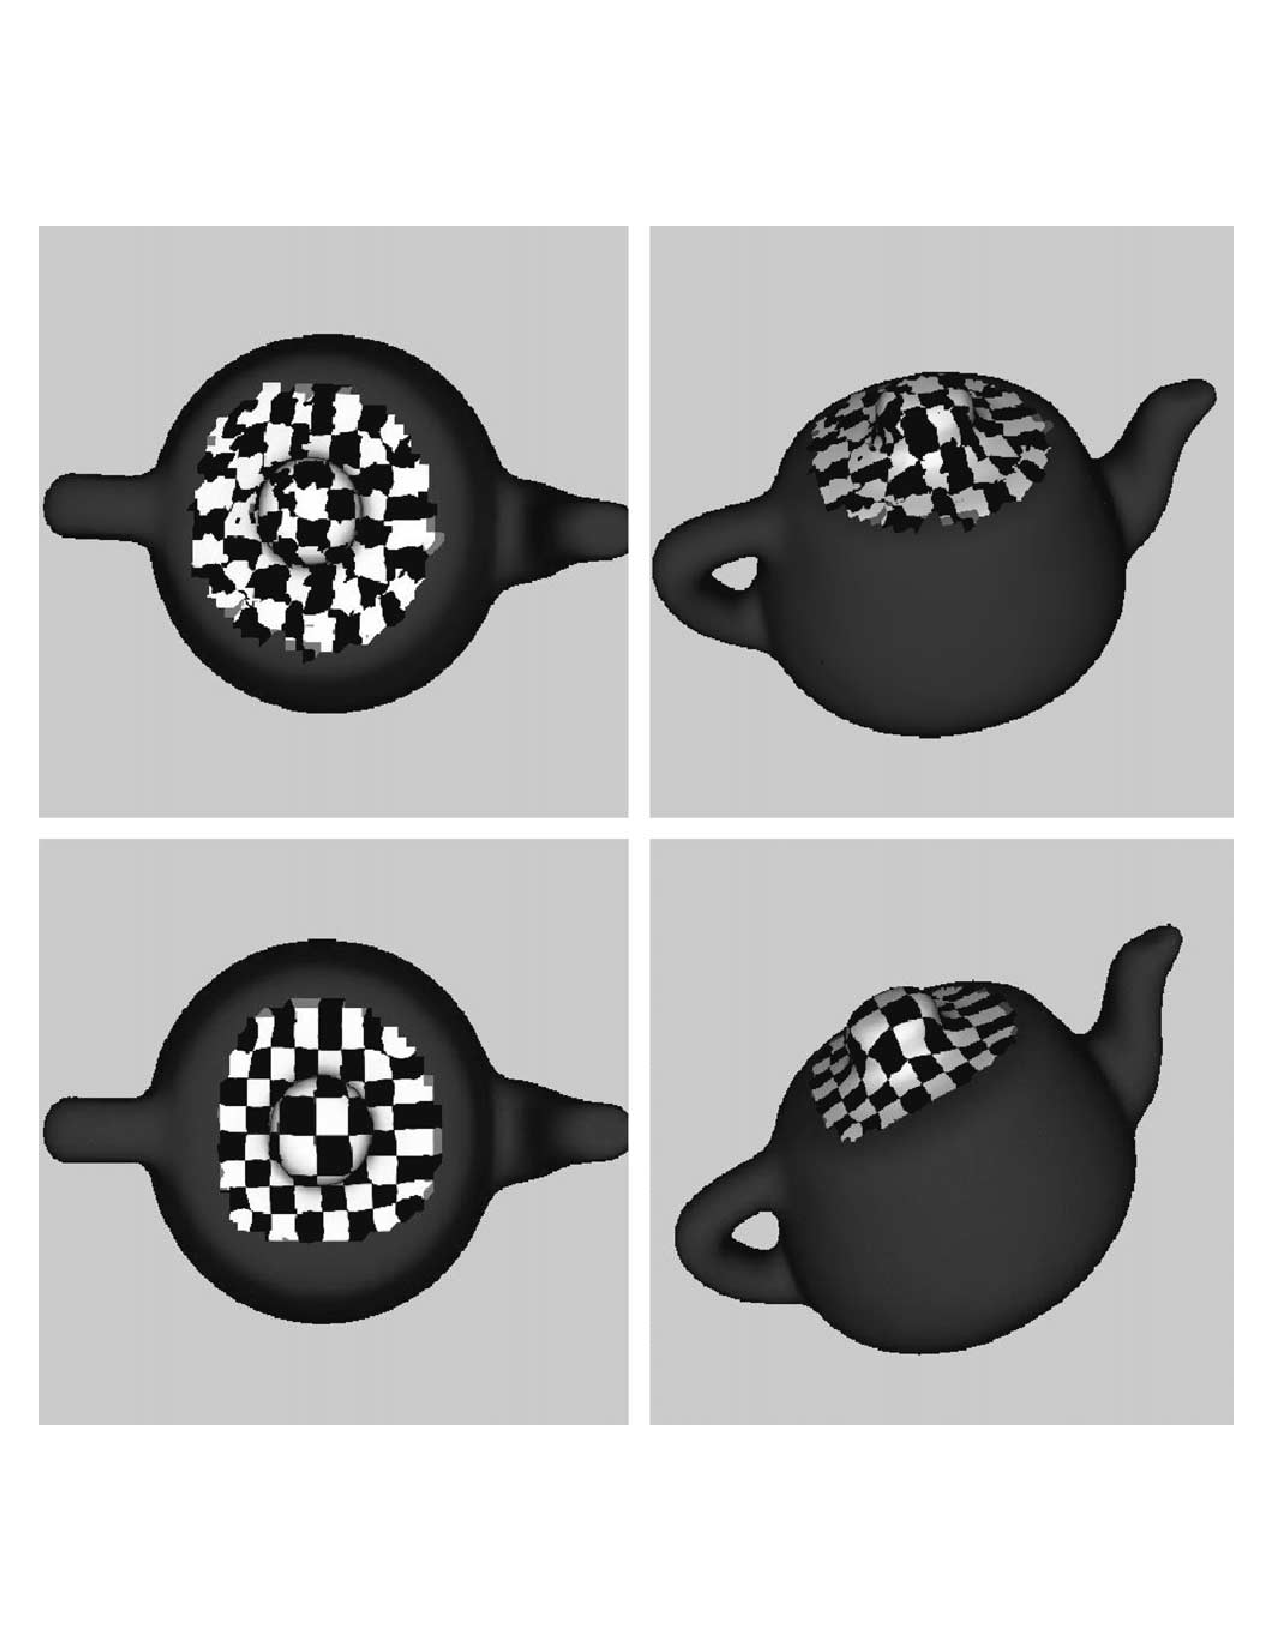
\includegraphics[scale=0.35]{teapot.pdf}
\end{figure}
\end{frame}


\begin{frame}{References}
\begin{thebibliography}{10}

\bibitem{Ber} M. Bertalm\'io, L.T. Cheng, S. Osher, G. Sapiro, 
\newblock {\it Variational problems and partial differential equations on implicit surfaces}, 
\newblock J. Comput. Phys. 174 (2) (2001) 759--780.\\

\bibitem{Mem} F. M\'emoli, G. Sapiro, S. Osher,
\newblock {\it Solving variational problems and partial differential equations mapping into general target manifolds}, 
\newblock J. Comput. Phys. 195 (2004) 263--292.\\

\bibitem{Ruu} S. Ruuth, B. Merriman,
\newblock {\it A simple embedding method for solving partial differential equations on surfaces}, 
\newblock J. Comput. Phys. 227 (2008) 1943--1961.\\

\end{thebibliography}
\end{frame}

\end{document}